\begin{figure}[httb!]
    \centering
    \begin{subfigure}{.45\textwidth}
        \centering
        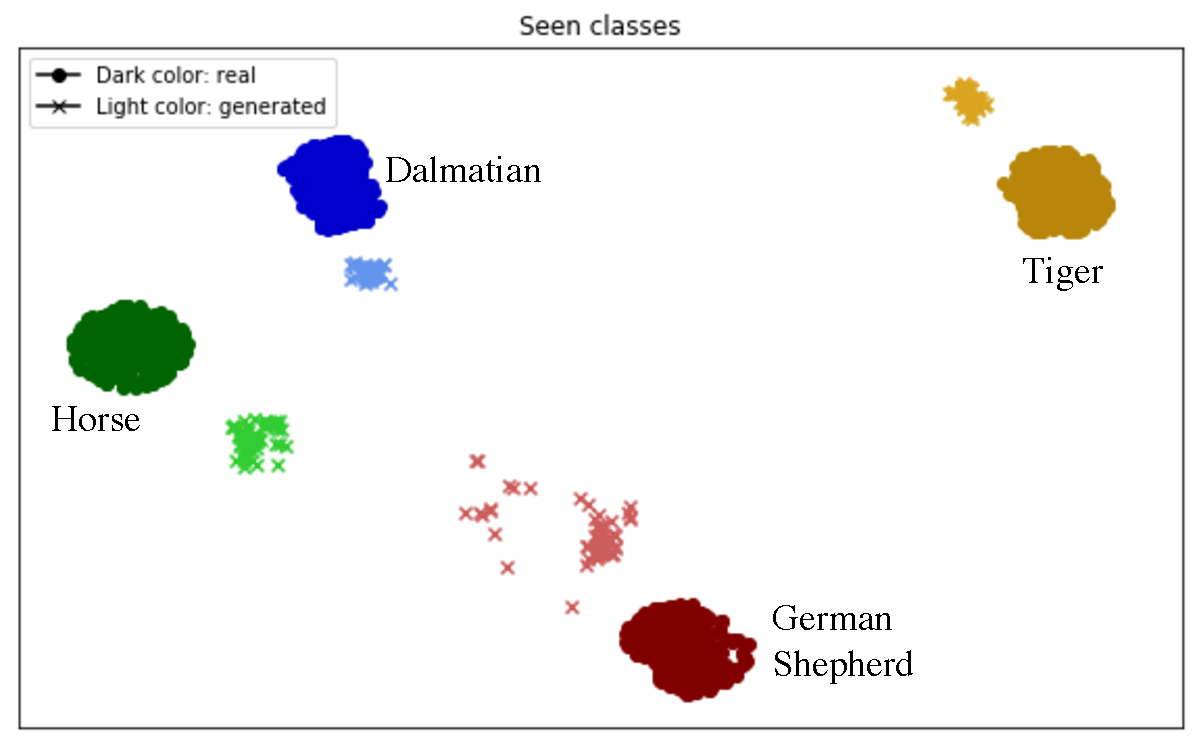
\includegraphics[width=\linewidth]{images/ghost/tsne_seen.pdf}
        \caption{Generator interpolation for \textit{seen} classes.}
        \label{fig:ghost_tsne_seen}
    \end{subfigure}%
    \hspace{1em}
    \begin{subfigure}{.45\textwidth}
        \centering
        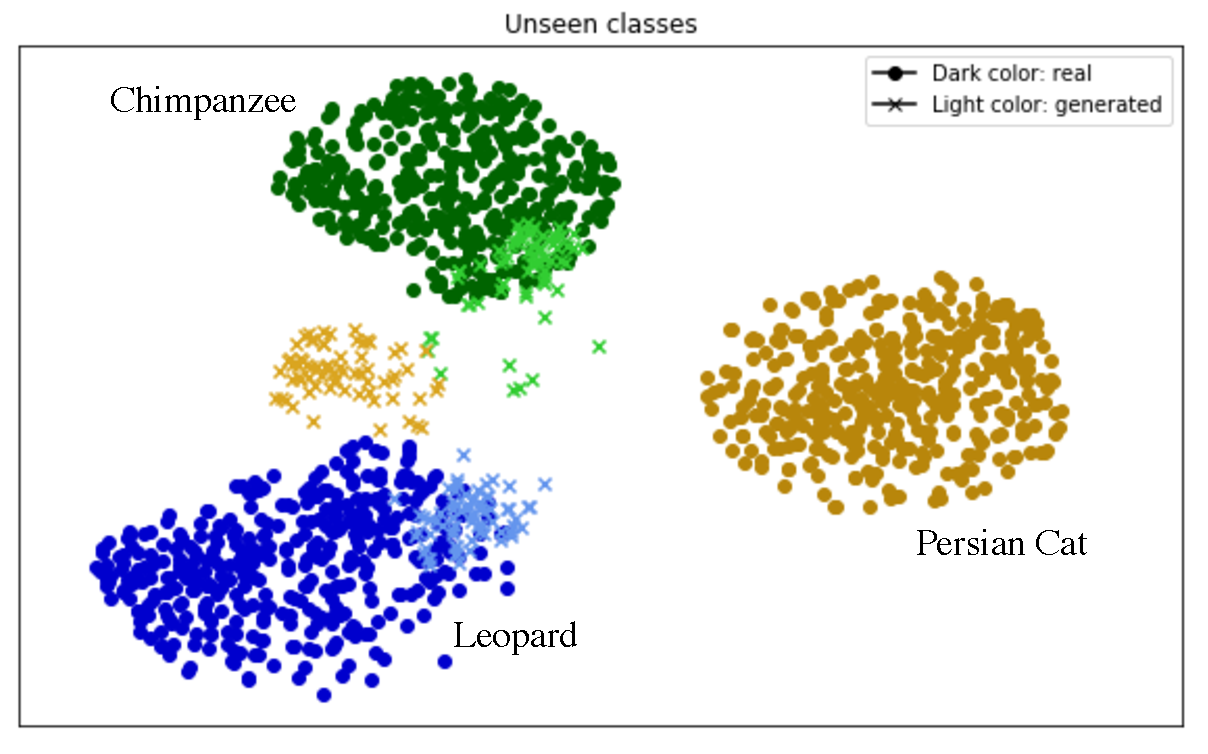
\includegraphics[width=\linewidth]{images/ghost/tsne_unseen.pdf}
        \caption{Generator extrapolation for \textit{unseen} classes.}
        \label{fig:ghost_tsne_unseen}
    \end{subfigure}
    \caption{\textbf{t-SNE of the latent space}. Dark colors indicate real features, while lighter colors denote their generated homologous. Real features extracted with $f^t$, and ghost features sampled from $g^t$. Generation in (a) is both well-located and tightly bound because the GMMN was trained to approximate those seen classes. In (b), the generator is asked to extrapolate to unseen classes only from their attributes, resulting in more spread features — still surprisingly, in general, well-located. Notice that the even the real features in (b) gets more spread, since the feature extractor was never trained on those classes.}
    \label{fig:ghost_tsne}
\end{figure}
